
As discussed before, the impact of variations and non-linearity of RRAM at the device level degrades sensing reliability and increases the read BER.
By sensing the discharge voltage $V_C$ multiple times, the proposed TSA can be easily extended to multi-level sensing. Fig. \ref{fig_multiple_sensing} illustrates a time-based 3-level sensing scheme, where the logic controller generates 3 enable pulses at different instants of time to PGI for successive sensing. Each of the enable pulse triggers one DFF to store the state, which contributes to the 3-bit thermometer code. Lastly, a thermometer code to binary code (T2B) decoder is used to convert the 3-bit thermometer code to a 2-bit binary code. The truth table of T2B decoder is listed in Fig. \ref{fig_multiple_sensing}(a).

The timing diagrams of critical nodes for RRAM in both LRS and HRS are depicted in Fig. \ref{fig_multiple_sensing}(b) with solid and dash lines respectively. The sensing points are $T_1$, $T_2$ and $T_3$ respectively, with a short enable time of $\Delta T$. In the first cycle, $Q[2:0] = 111 (000)$ for LRS (HRS). To show its robustness, the voltage margin of $V_C$ in the second cycle is narrowed because of variations. The sensing result $Q[2:0] = 011 (001)$ for LRS (HRS), from which we can still discriminate the states. For the single-point sensing, however, it is difficult to sense the state correctly -- if the sensing point is too early (like $CK[0]$), the output is high for both states; if the sensing point is too late (like $CK[2]$), the output is low for both states. This shows the advantage of multi-level sensing with more robust and higher accuracy.

Thanks to the features of time-domain processing, the overhead of the multi-level sensing scheme is only delay stages, compared with the conventional voltage or current mode multi-level sensing schemes. 
Multi-level sensing is beneficial to robust reading and can be applied to multi-level cell (MLC) sensing as well. Next, we will explain these separately.

\begin{figure}[!t]
\centerline
{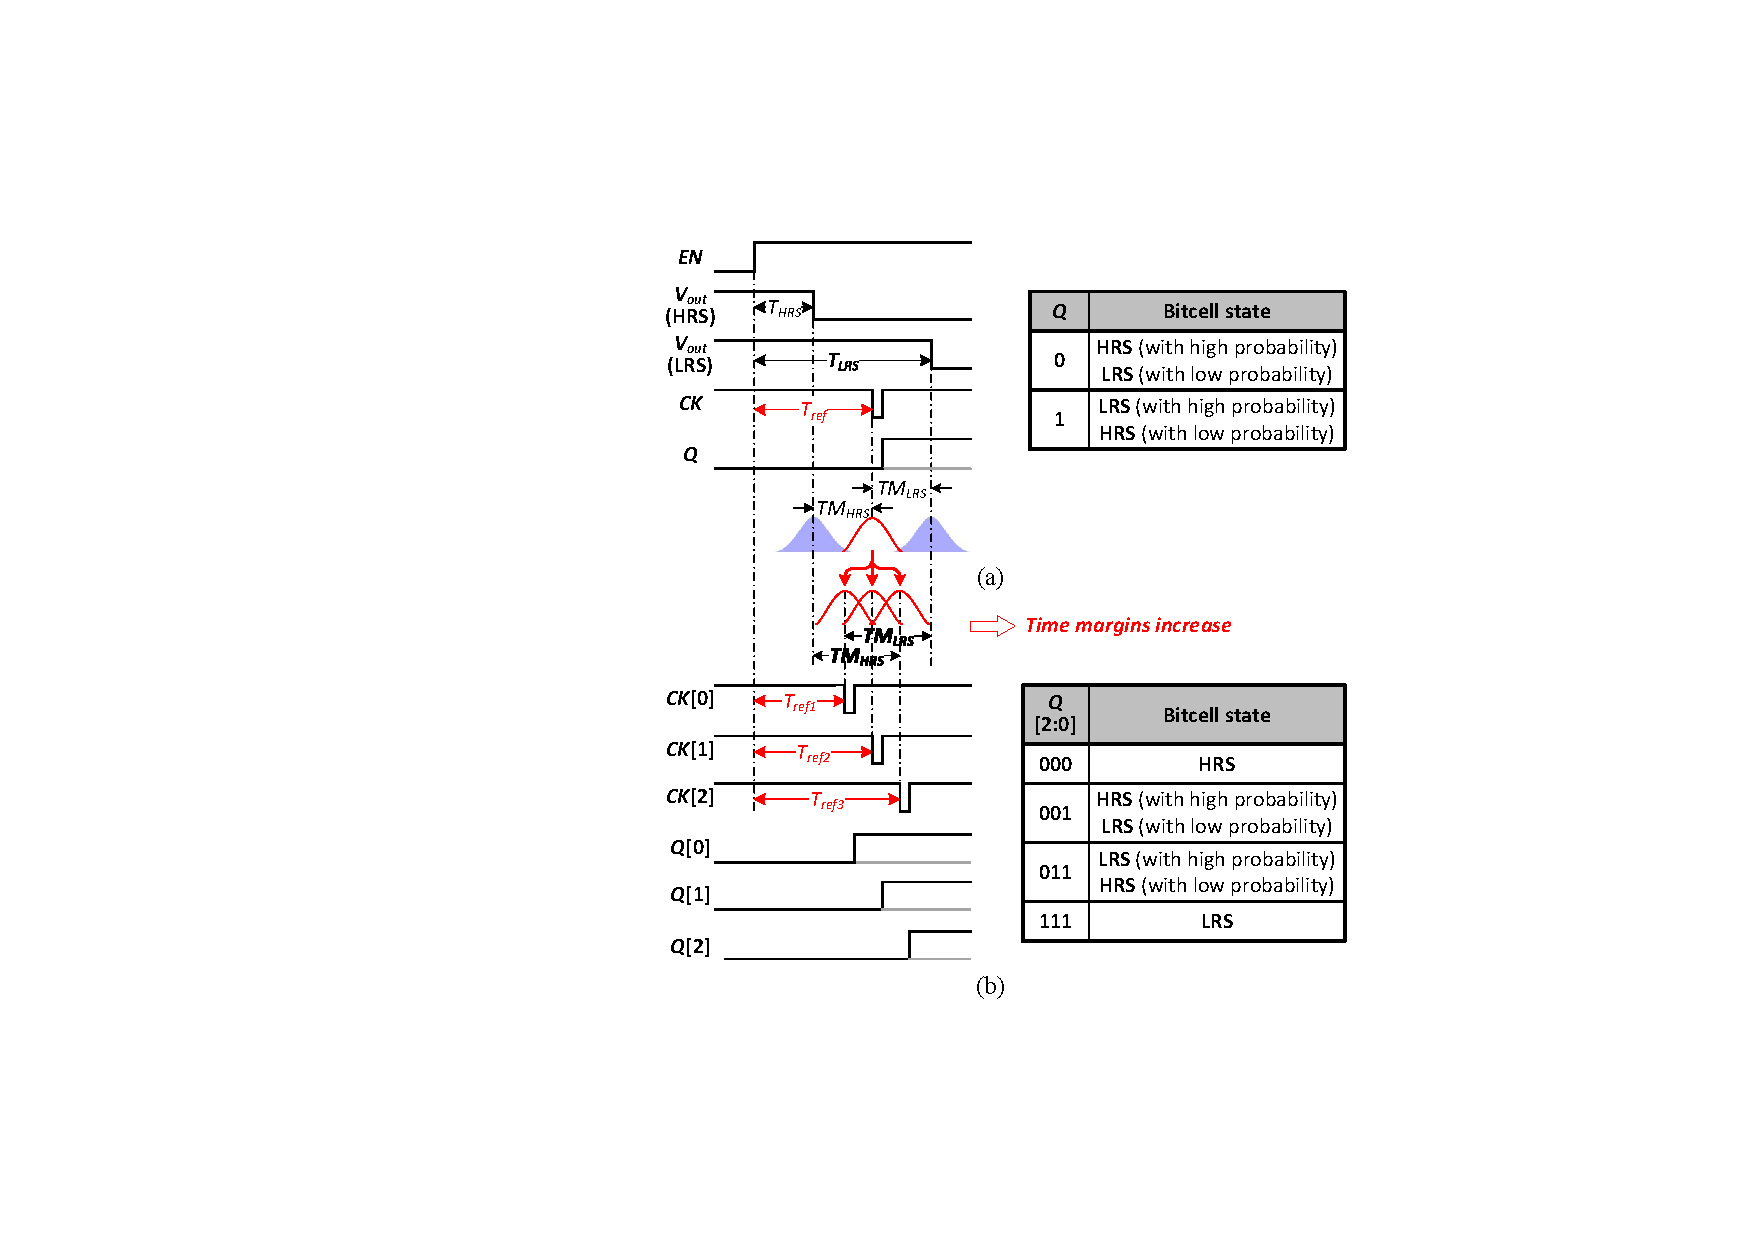
\includegraphics[width=0.46\textwidth]{fig/multi_level_sensing_waveforms_vs_conventional_new.pdf}}
\caption{Timing diagrams and bitcell state for (a) single sensing and (b) multiple sensing. The signal names are the same as Fig. \ref{fig_prop_circuit} and Fig. \ref{fig_multiple_sensing} respectively. Dashed lines represent HRS.}
\label{fig_MLS_compare}
\end{figure}

\subsection{Time-based Multi-level Sensing Technique}
% Conventional time-based sensing detects $V_{out,VTC}$ once and compares it with a reference delay signal $V_{EN,latch}$ to read the bitcell state, as shown in Fig. \ref{fig_sensing_mode}(c). However, the variations of $V_{out,VTC}$ induced by RRAM resistance variation and VTC variation may produce incorrect sensing. 
Conventional sensing schemes detect the state once and compare it with a reference signal to read the bitcell state. However, the fluctuations induced by RRAM resistance variation and sensing circuit variation may produce incorrect sensing. 
Fig. \ref{fig_MLS_compare}(a) shows the typical timing diagrams of a time-based single sensing scheme and the corresponding detection results of the bitcell state. 
To improve sensing accuracy and robustness, a multi-level sensing scheme is proposed, by which multiple points (3 in this case) are sensed consecutively, as shown in Fig. \ref{fig_multiple_sensing}.  
The reference signal is split into three references, assuming $T_{ref}=T_{ref2}$, as shown in Fig. \ref{fig_MLS_compare}(b). The bitcell state is represented by the 3-bit thermometer code $Q[2:0]$. If $Q[2:0]=00\times$, a HRS state is detected; and if $Q[2:0]=\times11$, a LRS state is detected. That is to say, the criteria for HRS are $T_{ref2}$ and $T_{ref3}$ -- the overall reference time $T_{ref,H}$ for HRS is longer than $T_{ref}$; the criteria for LRS are $T_{ref1}$ and $T_{ref2}$ -- the overall reference time $T_{ref,L}$ for LRS is shorter than $T_{ref}$. The time-based multi-level sensing scheme is actually converter the single reference in single sensing scheme to dynamic references -- shorter (longer) time reference for LRS (HRS) detecting. Therefore, both the time margins $TM_{LRS}$ and $TM_{HRS}$ increase. 

As discussed in section \ref{challenges}, $BER_{HRS}$ declines with longer reference time $T_{ref}$ and $BER_{LRS}$ declines with shorter reference time $T_{ref}$ (see  Fig. \ref{fig_BER_probability}). 
Compared to the single sensing scheme, both $BER_{HRS}$ and $BER_{LRS}$ are declined in the multi-level sensing scheme, resulting in a lower overall BER. This makes the multi-level sensing scheme more robust and accurate. 


\subsection{Application to Multi-level Cell (MLC) Sensing}

\begin{figure}[!t]
\centerline
{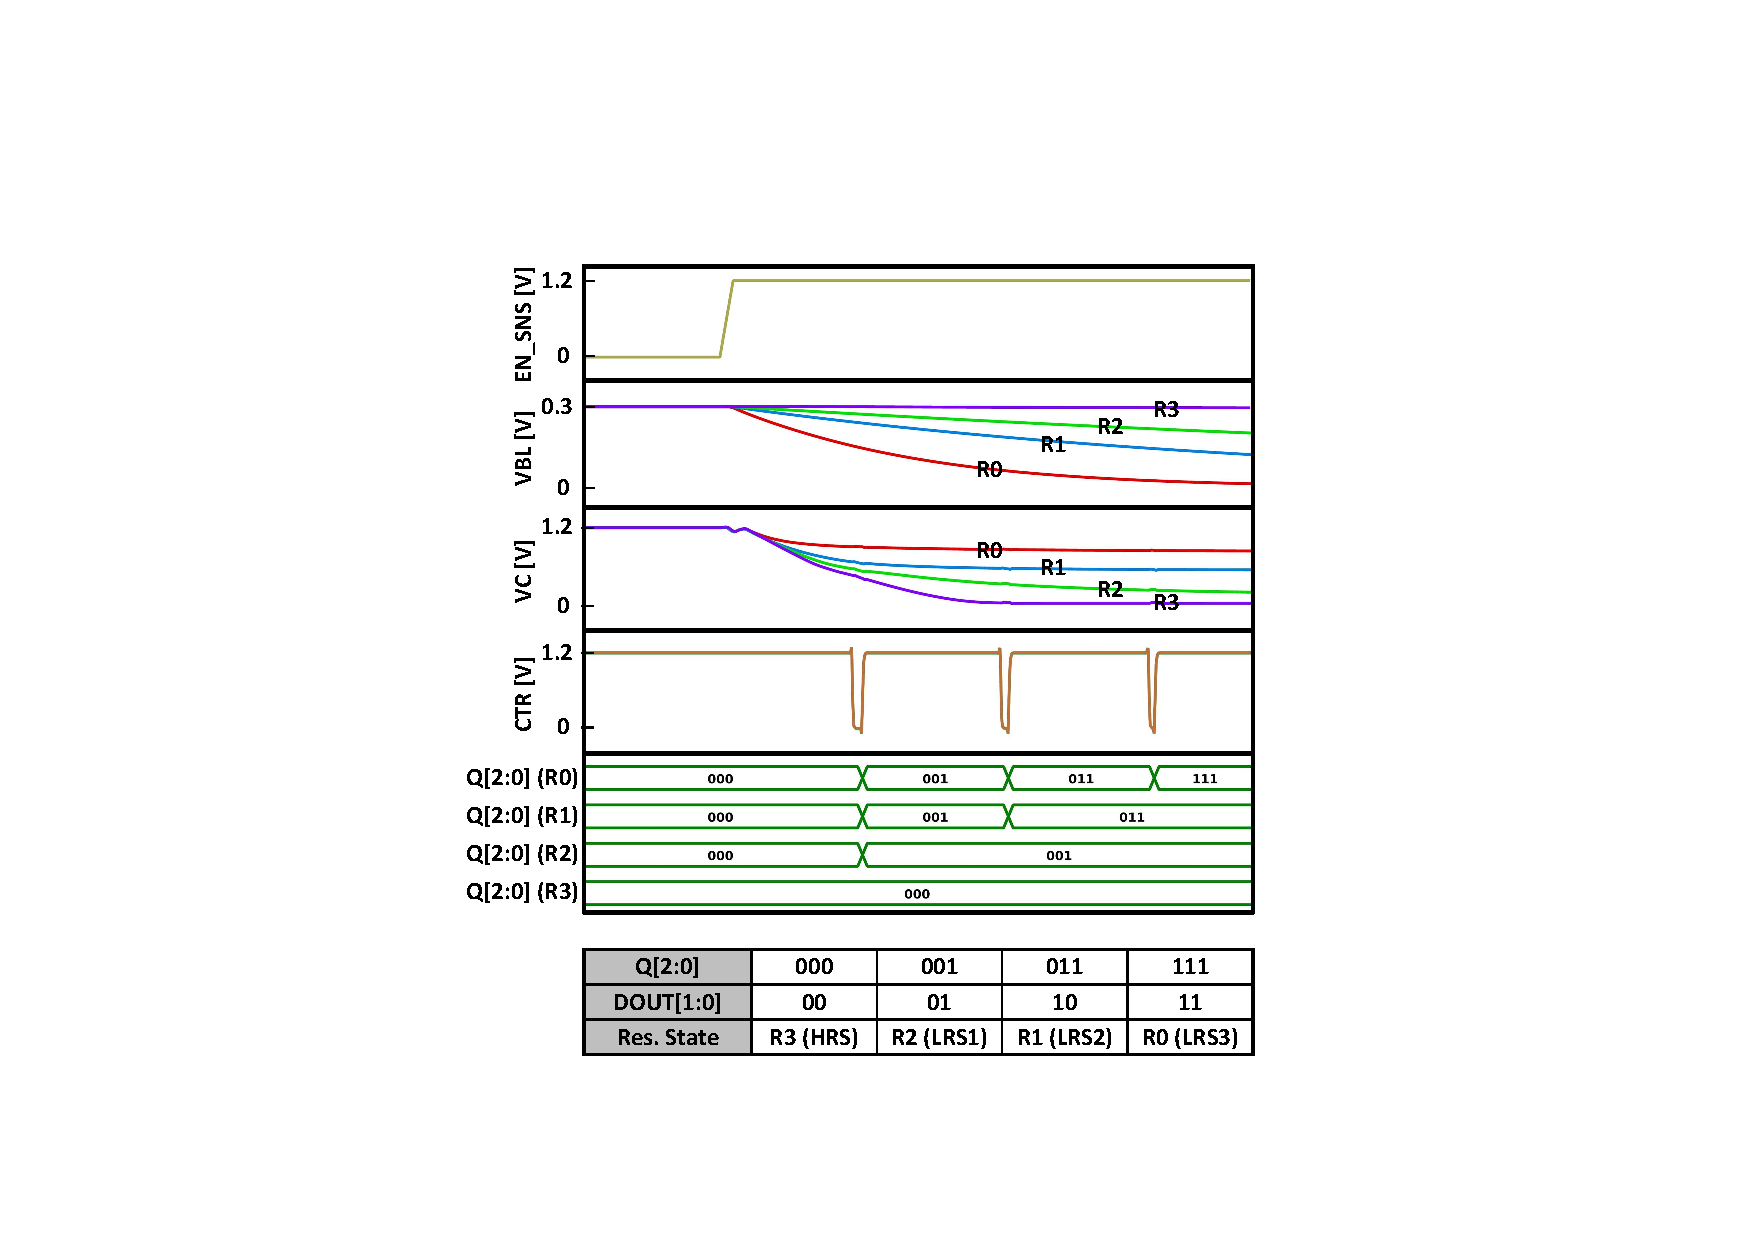
\includegraphics[width=0.49\textwidth]{fig/multi-level_sensing.pdf}}
\caption{Timing diagrams and bitcell states for 2-bit MLC RRAM sensing. The resistance decreases with the number of bit "1" detected in the output $Q[2:0]$.}
\label{fig_multi_level_sensing}
\end{figure}

The demand for increasing memory density has motivated researchers to store more bits per cell by implementing Multi-Level Cell (MLC) or multi-bit RRAM \cite{reuben2019time}.
MLC would be implemented by modulating (1) the compliant current, (2) programming voltage amplitude, or (3) programming pulse width \cite{prakash2016multilevel}.


% To simulate the BER for both HRS and LRS, the delay loop in Fig. \ref{fig_multiple_sensing} is broken to discharge $V_C$ freely. 
The proposed time-based multi-level sensing scheme also supports the detection of MLC RRAM. As an example, a 3-level consecutive sensing scheme can detect four different RRAM states (2-bit). Fig. \ref{fig_multi_level_sensing} depicts the sensing waveforms, the digital results, and the corresponding resistance states. 
Different resistance states develop different $V_{BL}$ levels (in this case, $R3>R2>R1>R0$), resulting in different discharge speeds of $V_C$. 
The state of MLC RRAM is detected by comparing voltage $V_C$ with trip voltage $V_{TRIP}$ of the subsequent inverter at three different times and decoding the latch results. The sensing results and the resistance states are listed at the bottom of Fig. \ref{fig_multi_level_sensing}.
In general, to sense $N$-bit MLC RRAM, the time-based sensing needs consecutively sense the state at $2^N-1$ time points. 
